
\chapter{Introducción}

\section{Antecedentes históricos}
El ser humano, en la década del 60, ante la incipiente necesidad de saber su posición en el planeta desarrolló un sistema de posicionamiento  llamado OMEGA y posteriormente otro llamado TRANSIT o \ac{NAVSAT}, que  fue resultado del trabajo conjunto de la NASA y el departamento de defensa de los Estados Unidos. Años después este acabó siendo reemplazado debido a la falta de precisión que este tenía, y que alcanzaba un error de hasta 250 metros.

Su sucesor apareció en la década del 70 bajo el nombre de \ac{GPS} y su precisión permitía posicionar un objeto con un error de menos de 5 metros. Esto a través del cálculo del tiempo que tarda en llegar la señal al receptor, es decir, el efecto Doppler.

Funciona actualmente con un mínimo de 24 satélites en órbita sobre la tierra cuyas trayectorias sincronizadas le permiten mapear completamente el planeta y entregar posicionamiento casi exacto a dispositivos móviles y vehículos.

Existen desde ya hace décadas intentos por emular lo logrado con el GPS, pero para espacios interiores, estos intentos han recibido el nombre de \ac{IPS}, que conforme a lo que se presentará en capítulos posteriores han logrado obtener resultados de posición con márgenes de error inferiores a los 3 m. 

\section{Definición del problema}
Las condiciones bajo las cuales es posible para la señal propagarse no se cumplen en todos los ambientes. Existen lugares en que a diferencia de lo que sucede en el exterior, donde la señal se refleja haciendo posible la triangulación de la posición, esta se absorbe parcial o completamente y principalmente corresponden a espacios interiores, tales como una bodega, un centro comercial o una oficina, haciendo que posicionarse dentro de estos espacios sea imposible a través del GPS, es por esto que a fin de brindar nuevas experiencias a usuarios a través del posicionamiento dentro de estos espacios se han desarrollado soluciones utilizando la banda de los 2.4 [GHz] que es la utilizada por, entre otros tecnologías, el Wi-Fi. 

Esta ha sido ampliamente estudiada debido a la alta penetración comercial que ha alcanzado precisamente en estos espacios donde el GPS no da cobertura, sin embargo, dentro de los distintos enfoques en que se han abordado los estudios se tiene que la medición de los niveles de potencia radiada desde los \ac{AP}, a través de los cuales se realiza la triangulación de la posición, se ven altamente afectados por la variación del escenario caracterizado. Este tipo de variaciones pueden ser inducidas por la presencia de personas u objetos que reflejen o absorban la señal.

Es por esto que el método a través del cual se de solución al problema del posicionamiento en interiores debe ser un \ac{IPS} capaz de compensar la incidencia de estas variaciones en el indicador de intensidad de señal recibida (RSSI) dentro de la operación del algoritmo y así, estimar correctamente la posición de objetivo deseado identificable a través de su dirección de \ac{MAC}.

\section{Estado del arte}

En cuánto a los enfoques que se han considerado para evaluar la posición de un dispositivo móvil en un espacio interior se han podido desarrollar diversas soluciones que apuntan de una u otra manera a aproximaciones geométricas. A fin de ordenar según la técnica, la documentación consultada, se hará una clasificación y dentro de las categorías, explicará las investigaciones en el área.\\

%%%%%%%%%%%%%%%%%%%%%%%%%%%%%%%%%%%%%%%%%%%%%%%%%%%%%%%%%%
                \clearpage 
%%%%%%%%%%%%%%%%%%%%%%%%%%%%%%%%%%%%%%%%%%%%%%%%%%%%%%%%%%

Se abordará siguiendo el esquema que está a continuación:
\begin{figure}[h!]
    \centering
    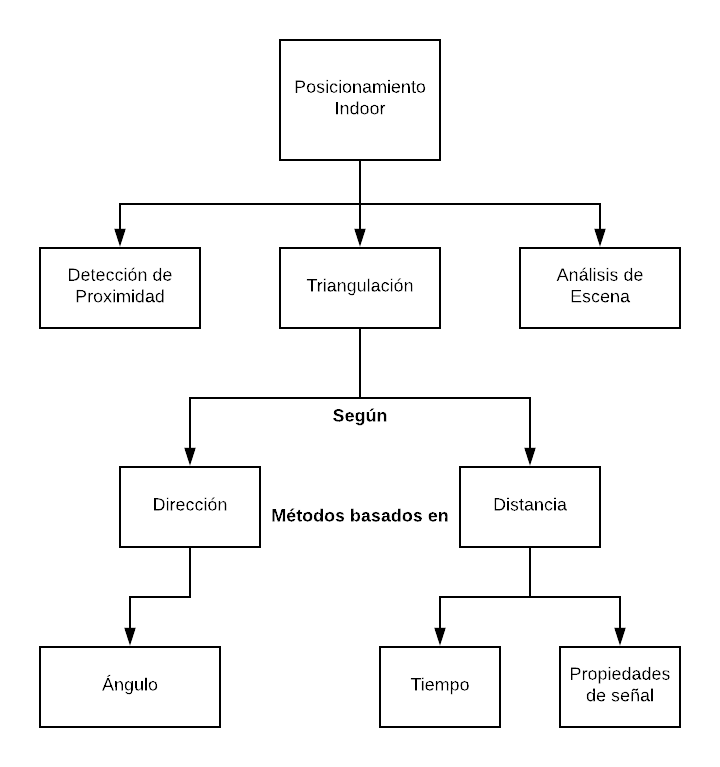
\includegraphics[scale = 0.3]{./images/diagrama}
    \label{fig:diagrama}
\end{figure}

Así, comenzando por el tipo de algoritmos basados en \textit{Detección de proximidad} se tiene que de acyerdo a lo visto en \cite{6}, algunas de las tecnologías que permiten esto, es aquella asociada al uso de beacons; pequeños dispositivos capaces de emitir señales de onda corta por medio de la tecnología Bluetooth, y que puede llegar hasta 50 metros de alcance. Es precisamente en el uso de estos dispositivos que en \cite{20}, los autores, con el fin de integrarlos a tecnologías del IoT, hacen todo un estudio respecto de los distintos tipos de beacons que existen en el mercado, haciendo énfasis en las características asociadas al consumo de energía, al uso del ancho de banda, y de la latencia asociada a la respuesta de los beacons del tipo \ac{BLE}.\\

Presentan además como es que se han integrado estos dispositivos en el comercio, museos, hospitales y estaciones de trabajo, permitiendo así, el surgimiento potencial de una industria interesada en sus bondades. Explican allí que el uso de los beacons se traduce en que cada dispositivo posee una etiqueta única, que para efectos de este trabajo bien puede ser la dirección \ac{MAC}, que al comunicarse con el dispositivo móvil permite a este, enviar una respuesta de cuáles dispositivos tiene a la vista y entonces, comparar el \ac{RSS} para así estimar respecto de cuál beacon está más cercano el usuario.\\

\begin{figure}[h!]
    \centering
    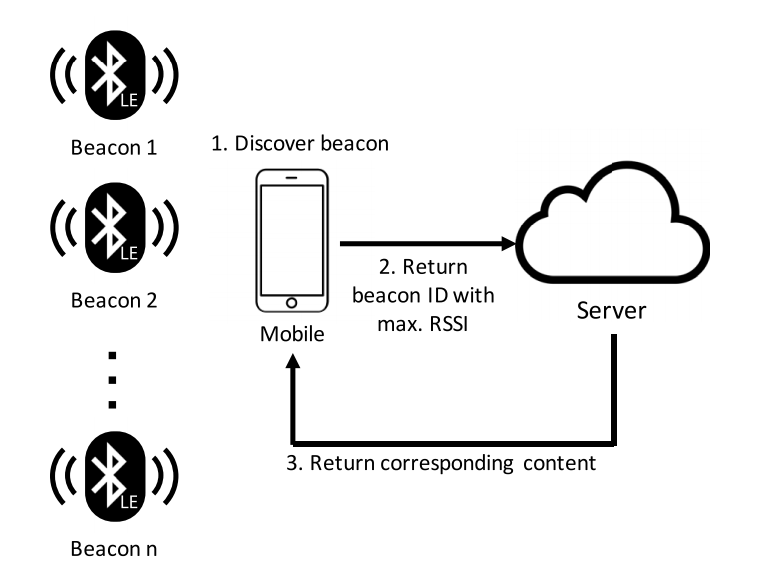
\includegraphics[scale=0.3]{./images/beacon}
    \caption{Imagen de la comparación de la cercanía según el nivel de RSS según un sistema basado en la interacción de beacons BLE}
    \label{fig:my_label}
\end{figure}

Sin embargo, pese a las ventajas asociadas el uso de estos dispositivos, se tiene que así como señalan en \cite{1}, la principal desventaja de algoritmos basados en tecnologías por proximidad, es que generalmente se requiere de hardware adicional, en lugar de los dispositivos que ya se usan e instalan para proveer de internet a usuarios. Además, hay que tener en cuenta que el hardware para este tipo de implementaciones hace uso de una parte no licenciada del espectro, por lo que es altamente susceptible a ser afectada por interferencias de equipos funcionando en la misma banda.\\

Luego, en el tipo de algoritmo basados en \textit{Análisis de Escena} los autores en \cite{1}, presentan un sistema de posicionamiento indoor para navegación que puede funcionar indistintamente si se trata de un smartphone o de una tablet, en tanto se puedan usar los sensores que ya se incluyen en el funcionamiento interno de este. Para el reconocimiento de escena conciben el sistema como uno de dos partes \cite{8}; una offline, que consiste en la extracción de características del entorno y un posterior almacenamiento en una base de datos que servirá para comparar las medidas que se obtengan en la etapa online.Durante esta etapa, la información recolectada es usada par obtener la posición estimada.\\

Las dificultades principales a las que se ven enfrentados estos métodos son los movimientos estructurales a las cuales los espacios se ven sometidos, ya que esto elimina puntos de referencia por simples movimientos de un lugar a otro, lo que conlleva una calibración y medición periódica.\cite{20}\\

Finalmente, en lo que respecta al algoritmo de \textit{Triangulación} se deben hacer algunas subclasificaciones a fin de dejar más claro cómo se ha abordado el problema, de esta manera se tiene que para los métodos basados en:\\
\begin{enumerate}
\item{\textbf{Triangulación:}
    \begin{itemize}
        \item{\textbf{\ac{AoA}}: Referido, como su nombre lo dice, se refiere al ángulo de llegada de la señal del dispositivo móvil, proveniente de una ubicación desconocida, la cual es recibida en múltiples estaciones base. Este algoritmo es evaluado por diversos autores; en \cite{1} los autores lo trabajan como un complemento al uso de los sensores propios del dispositivo, logrando una performance destacable en cuánto a la media del error, sin embargo, no presentan resultados numéricos que permitan conocer el área de cobertura, así como la disponibilidad.\\
            
        En \cite{20}, señalan que una de las desventajas de este método radica en que debido a que no todos los dispositivos están en línea vista con el equipo receptor, la precisión de las mediciones se degrada, haciendo incapié en que la disposición del arreglo de antenas emisoras juega un rol fundamental en estimar la posición.\\
            
        En \cite{21} comienzan señalando que si bien existen otros algoritmos tales como ToF o TDoF, mucho menos complejos que el de AoA, si es posible implementar un método que alcance una buena precisión pese a las imprecisiones en las mediciones de ángulo y el bajo número de beacons dispuestos. No obstante, en \cite{5} los autores hablan de aproximaciones  híbridos que trabajan con lo mejor de los algoritmos basados en tiempo, y en ángulo para reducir la complejidad que introduce el ambiente indoor. Sin embargo, no logran reducir ni el número de antenas ni el ancho de banda utilizado.}
        \end{itemize}
        }
\item{\textbf{Trilateración}:Este algoritmo puede ser abordado a través de distintas técnicas, algunas de ellas son:
        
    \begin{itemize}
        \item{\textbf{\ac{ToF}}: este concepto está referido a la técnica a través de la cual se realizan cálculos de posición a través del tiempo de llegada de la señal respecto de diversos puntos de referencia.\cite{5}\\
            
        Algunas de las dificultades que exponen los autores en \cite{22} es que la medición de la señal basada en el  tiempo de propagación es que requiere señales de \ac{UWB}, lo que lleva a un consumo de energía considerable, que no ofrece mayor precisión en largas distancias. Muy por el contrario, la precisión de la medición es directamente proporcional a la distancia, pudiendo alcanzar detalle de centímetros cuando la distancia es corta, pero fallas considerables si es que la señal ultrasónica debe viajar sufriendo las atenuaciones del aire así como del efecto multitrayectoria.\\
            
        No obstante, en el sistema \textit{TWINS} de \cite{2} los autores lograron montar un sistema basado en este algoritmo donde utilizan un rango de dos vías, aprovechando el intercambio de tráfico de DATA/ACK, que luego de sortear problemas asociados al protocolo de comunicación, esto es:  ajustar la frecuencia de trabajo, sincronizar los equipos para que funcionen en un mismo tiempo, les permite posicionar usuarios que pueden moverse libremente por el espacio delimitado por el sistema.}\\
        
        \item{\textbf{\ac{RSSI}}: A través de esta técnica los autores en \cite{3} y \cite{4} relacionan los niveles de \ac{RSS} desde los \ac{AP} existentes con la distancia que hay a un AP particular. A través de los modelos de propagación pueden hacer una regresión que, cuando se ha calculado la distancia que hay a los, como mínimo 3, AP se puede entonces crear un sistema de ecuaciones cuyas soluciones son las coordenadas espaciales del objetivo.\\
        
        Otra técnica, algo menos acabada en comparación a lo visto anteriormente, es aquella vista en \cite{13} que hace uso de los niveles de potencia recibida de cada uno de los AP para caracterizar un espacio interior y así, hacer un sistema de coordenadas que permita estimar la posición del usuario. Sin embargo, conocidas las propiedades de los espacios indoor, es sabido que estos son muy dinámicos, que cualquier superficie puede reflejar y absorber potencia, haciendo así variar estos niveles e inducir un margen de error que posicione erróneamente al usuario.\\
        
        Un algoritmo basado en \ac{RSSI}, pero que no usa propiedades geométricas para hacer el posicionamiento es aquell llamado \textit{Fingerprinting Based Indoor Localization}, en \cite{6} los autores lo presentan como una técnica que consiste en dos etapas; la primera, conocida como offline, es la de hacer una colección de los niveles de potencia recibidos en las distintas áreas de interés y almacenarlas en una base de datos que sirva de entrenamiento para las predicciones en las cuales se basará la etapa siguiente; luego, en la etapa \textit{online}, lo que se busca es medir los niveles de potencia y compararlos con el vector de \ac{RSS} que más se le parezca.\\
        
        Para esto, la etapa offline puede verse apoyado por herramientas estadísticas como las de los trabajos \cite{8}, \cite{10},\cite{11},\cite{12} y \cite{14}, o bien, por algoritmos basados técnicas de reconocimiento de patrones probabilísticas y determinísticas tales como KNN, RN, SVM, RNN u otros.\\
        
        \begin{itemize}
            \item {\textbf{\ac{KNN}}: Este algoritmo introducido teóricamente en \cite{7} aparece como un método que autores en \cite{23} usaron KNN para eliminar aquellos puntos individuales en el dataset de muestreo, que bien podría corresponder a aquellos vectores que surgieron de capturar más AP. Luego, usaron SVM para posicionar al usuario. En este trabajo los resultados muestran que el algoritmo híbrido mejora considerablemente la precisión y la velocidad de este.\\
            
            A diferencia de el trabajo anterior, en \cite{24} lo usan para directamente obtener la posición del dispositivo, a la vez que en \cite{25} señalan que el comportamiento de KNN superó en términos de precisión al más sofisticado algoritmo basado en un modelo probabilístico.\\}
            
            \item {\textbf{\ac{RNN}}: \label{RNN} En \cite{15} señalan que las RNN han sido usadas como algoritmos de clasificación en diversas aplicaciones, debido a que puede manejar varias series de datos de tiempo, pero que actualmente no han habido investigaciones que asocien sistemas de posicionamiento indoor al uso de este algoritmo.\\
            
            Por este motivo, ellos desarrollaron un sistema que se basa en RNN y que permite clasificar pares ordenados \textit{(x,y)} basados en el RSSI de cada sensor. Específicamente para implementar un tipo de regresión que permite predecir las coordenadas al considerar cada AP como nodo. Algo parecido a lo que se deseaba conseguir en el trabajo presentado en \cite{28}.\\}
            
            \item {\textbf{\ac{RNA}}: En se \cite{26} aborde el problema de posicionamiento indoor a través del mismo enfoque visto anteriormente en \ref{RNN}, es decir, se busca transformar los RSS a distancias y así determinar las coordenadas del objetivo. La diferencia radica en que acá no se usan AP, sino que otra tecnología llamada ZigBee que también actúa como un sensor de red, señalando que el uso de este, en conjunto con el modelo, trabajan sustancialmente mejor que la técnica de triangulación que por si sola es inestable.\\
            
            Por otro lado en \cite{27} las personas de la investigación comentan que en investigaciones anteriores o en general, en los trabajos que buscan determinar la posición basándose en una ANN utilizan características del ambiente de la \ac{WLAN} para caracterizarlo, estas pueden ser: RSS, que es lo más recurrente a la hora de abordar estos problemas, o bien, \ac{SNR} de los múltiples AP a fin de mapear el espacio en la etapa offline. En contraste a lo anterior señalan que su trabajo es capaz de alcanzar una precisión del 92.86\% solo con el uso de una red de apenas 3 capas que permiten posicionar con una exactitud de tres metros sin incurrir en un margen de error importante, recalcando que si se realiza una división por área, entonces la performance del sistema mejora considerablemente y cuyos resultados fueron contrastados a través de KNN.\\
            
            Finalmente en \cite{28}, al igual que en \cite{27} utilizaron una ANN que se compuso de y capas, y estas a su vez, se desglosaron en 1 capa de entradas, 3 capas ocultas, con 28 nodos cada capa, y 1 de salida, con dos nodos. Interesante señalar que el resultado de agregar 2 capas se tradujo en alcanzar una precisión de 2 metros, que lleva a la conclusión de que la precisión guarda cierta dependencia con el número de nodos y capas ocultas.\\}
        \end{itemize}
        }
    \end{itemize}
        }
\end{enumerate}


%%%%%%%%%%%%%%%%%%%%%%%%%%%%%%%%%%%%%%%%%%%%%%%%%%%%%%%%%%
                \clearpage 
%%%%%%%%%%%%%%%%%%%%%%%%%%%%%%%%%%%%%%%%%%%%%%%%%%%%%%%%%%

\section{Hipótesis de trabajo}
\begin{center}
\textit{''Es posible posicionar un dispositivo, identificable a través de su MAC, en un espacio interior utilizando una Red Neuronal Artificial para compensar las variaciones de RSS de los \ac{AP} usados en la trilateración''}
\end{center}

\section{Objetivos}
A continuación se señalan los objetivos que apuntan a resolver el problema presentado y a probar la hipótesis de trabajo.

\subsection{Objetivo general}
Posicionar un dispositivo móvil, reconocible a través de su \ac{MAC} dentro de un espacio interior, a través de algoritmos de trilateración y \ac{RNA}.

%\section{Objetivos específicos}
%\begin{enumerate}
%\item{a}
%\end{enumerate}

\section{Alcances y limitaciones}
El alcance de este proyecto estará limitado a encontrar la posición de un dispositivo móvil dentro del espacio del segundo piso de Edificio Tecnológico Mecánico de la Universidad de Concepción. Se ejecutará el algoritmo desarrollado en una laptop personal, utilizando Raspberry Pi como \ac{AP} y el resultado del posicionamiento se desplegará en una interfaz gráfica desarrollada en python.

\section{Metodología}

Para lograr posicionar un dispositivo móvil dentro del espacio interior, se buscará en primera instancia extraer los datos de RSSI obtenidos desde las tarjetas de Red de las placas. Posterior a esto se caracterizará el espacio de trabajo con sus respectivos niveles de RSS. Estas serán usadas para entrenar un modelo que, a través de RNN, pueda detectar la posición en que se halla un usuario, respecto de los niveles de potencia y la certidumbre que arroje el entrenamiento realizado. Finalmente, el resultado será desplegado en una interfaz gráfica.